\subsection{SM4默认轮函数连续异或与减少指令依赖}
在默认循环实现版本中每轮循环都有\texttt{tmp = X1 \^ X2 \^ X3 \^ rk[i]},由于异或操作满足结合律:
\[ a \oplus b \oplus c \oplus d = (a\oplus b) \oplus (c \oplus d)  \]
因此这里可以分别计算前前两个变量的异或结果和后两个变量的异或结果,分别存到临时变量中,最后将这两个临时变量再求异或,这样能减少指令之间的依赖性,即可以同时求两个临时变量。否则,连续异或时想要求后一个异或必须要等前一个异或运算结束,指令依赖关系导致只能串行执行。
在SM4每轮最后的换位赋值时可能产生写寄存器又马上读的依赖,因此可以用临时变量存放$X_1,X_2$值,这样能确保整个过程只发生寄存器移动而无需内存访问。具体代码如下:
\begin{lstlisting}[title={openhitls/testcode/demo/sm4\_reduced\_dep.c}]
static void sm4EncryptBlock(const uint32_t rk[32],
                            const uint8_t in[16],
                            uint8_t out[16])
{
    uint32_t X0, X1, X2, X3;
    {
        uint32_t arr[4];
        sm4LoadBlock(in, arr);
        X0 = arr[0]; X1 = arr[1]; X2 = arr[2]; X3 = arr[3];
    }

    for (int i = 0; i < 32; i++) {
        /* Break the XOR chain: X1^X2 and X3^rk are independent */
        uint32_t tmp1  = X1 ^ X2;
        uint32_t tmp2  = X3 ^ rk[i];
        uint32_t tmp   = tmp1 ^ tmp2;
        uint32_t t     = sm4T(tmp);
        uint32_t newX0 = X0 ^ t;

        /* Feistel rotation with temporaries */
        uint32_t prevX1 = X1;
        uint32_t prevX2 = X2;
        X0 = prevX1;
        X1 = prevX2;
        X2 = X3;
        X3 = newX0;
    }

    {
        uint32_t arr[4] = {X0, X1, X2, X3};
        sm4StoreBlock(arr, out);
    }
}
\end{lstlisting}
编译运行结果如图:
\begin{figure}[H]
    \centering
    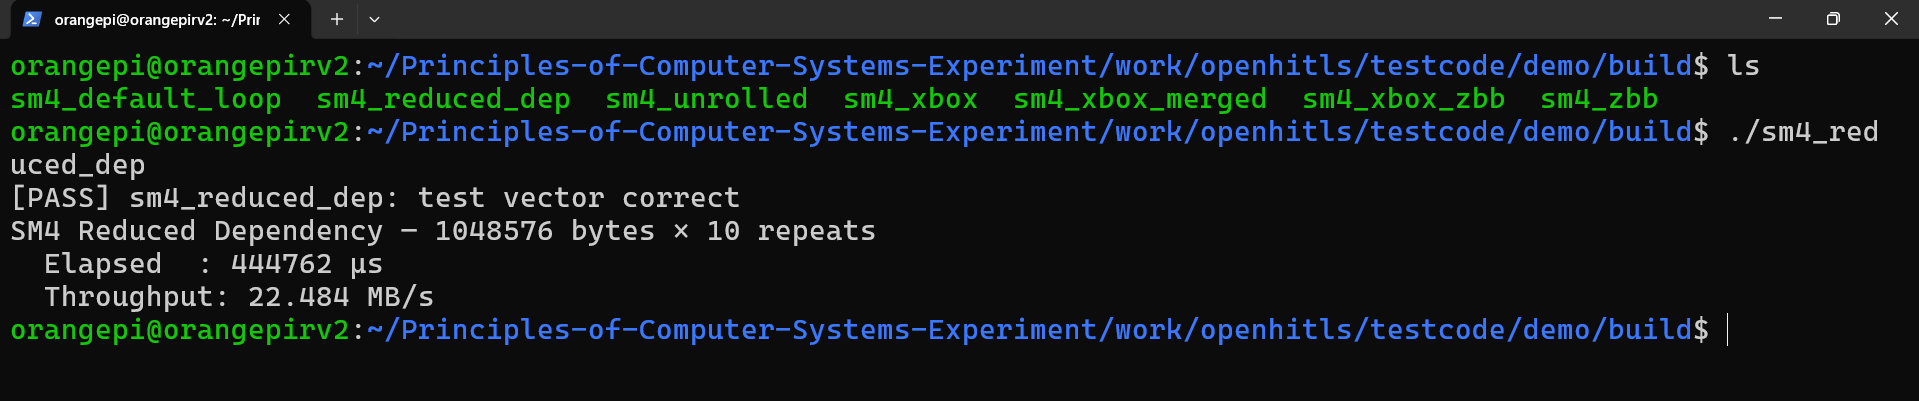
\includegraphics[width = 1\textwidth]{figure/sm4_reduce_dep.png}
    \caption{SM4减少指令依赖}
\end{figure}
可以看到程序运行效率和吞吐量较默认循环版几乎相同,优化非常有限。